\documentclass{standalone}
\usepackage{tikz}
\usetikzlibrary{patterns, angles, quotes}

\begin{document}
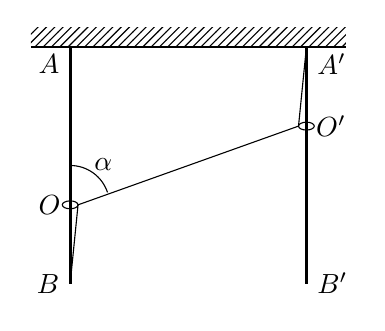
\begin{tikzpicture}
	\coordinate (A) at (0.5, 0);
    \coordinate (O) at (0.5,-2);
    \coordinate (Oprime) at (3.5,-1);
    
	\draw [draw=none, pattern=north east lines] (0,0) rectangle (4,0.25);
	\draw [thick] (0,0) -- (4,0);
	\draw [very thick] (A) node [below=6pt, left]  {$A$} -- (0.5, -3) node [left] {$B$};
	\draw [very thick] (3.5, 0) node [below=6pt, right]  {$A^{\prime}$} -- (3.5, -3) node [right]  {$B^{\prime}$};
	\draw (3.5, 0) -- (3.4, -1) -- (0.6, -2) -- (0.5, -3);
	\draw (O) ellipse (0.1 and 0.05) node [left] {$O$};
	\draw (Oprime) ellipse (0.1 and 0.05) node [right] {$O^{\prime}$};
	\pic [draw, -, angle eccentricity=1.5] {angle = Oprime--O--A};
	\node [right=12pt, above=9pt] at (O) {$\alpha$};
\end{tikzpicture}
\end{document}